\documentclass[11pt]{amsart}
\usepackage{geometry}                % See geometry.pdf to learn the layout options. There are lots.
\geometry{letterpaper}                   % ... or a4paper or a5paper or ... 
%\geometry{landscape}                % Activate for for rotated page geometry
%\usepackage[parfill]{parskip}    % Activate to begin paragraphs with an empty line rather than an indent
\usepackage{graphicx}
\usepackage{amssymb}
\usepackage{url}
\usepackage{epstopdf}
\usepackage{setspace}
\DeclareGraphicsRule{.tif}{png}{.png}{`convert #1 `dirname #1`/`basename #1 .tif`.png}

\title{STA 250 HW1: Bayes Module}
\author{Christopher Conley}
\date{}                                           % Activate to display a given date or no date

\begin{document}
\maketitle
\tableofcontents
\onehalfspacing

\section*{Question 2: Logistic regression on simulated data}
\subsection*{Analytic form of the posterior distribution (up to proportionality)}

The prior is normally distributed with density: 
\[ p( \beta)  = (2\pi)^{-p/2} |\Sigma_0| ^ {-1/2}  exp \{ -\frac{1}{2}  (\beta - \mu_0)^T \Sigma_0^{-1/2}  (\beta - \mu_0) \}\]

where $\mu \in \mathbb{R} $ and $\Sigma_0$ is positive definite. The likelihood on $n$ grouped covariates is expressed as:

\[ p( y | \beta ) = \prod_{i = 1}^n \binom{m_i}{y_i} \text{expit}( X \beta)^{y_i} \times \{1 - \text{expit}( X \beta) \}^{m_i - y_i} \]

So the posterior has the form.

\[ p( \beta | y) \propto p (\beta) \times p(y | \beta ) \]

If we cancel and ignore constants, the log posterior (up to proportionality)may be expressed in simpler form: 

\[ p( \beta | y) \propto -\frac{1}{2} \beta^T \Sigma_0^{-1/2} \beta + \beta^T \Sigma_0^{-1/2} \mu_0 + 
                                        \sum_{i = 1}^n \Big( y_i * x_i^T \beta - m_i log \{ 1 +   \text{expit}( x_i^T \beta) \} \Big )  \]

where it is easy to see the sufficient statistic, $y^TX$ in the likelihood. 

\subsection*{The Metropolis Within Gibbs Sampler (MWG)}

There is no analytic form of the full conditionals of $p( \beta_1 | \beta_0, y), p( \beta_0 | \beta_1, y)$, which makes a vanilla Gibbs sampler intractable.  A MWG algorithm was implemented such that the sampling process was guided by the Metropolis Hastings decision rule for each target parameter,  $\beta^{(t)}_j$, and conditioned on previously sampled (accepted or rejected) target parameters, $\beta^{(t)}_{1:(j - 1)}$, within each time point of the chain.  The following table describes key specifications of the MWG implementation. 

%\begin{table}[htdp]
%\caption{default}
%\begin{center}
\begin{tabular}{ll}
\hline
Component & Description \\
\hline
Proposal Distribution & $Normal(\beta^{(t)}_j, \nu_j)$ for $j = 1, \dots, p$\\ 
Tuning Process of $\nu$ & Adaptive MCMC, retune every 100 iterations \\
Post Burn-in Chain Length & 20,000 \\
Burnin Length & 5,000 \\
Prior Initialization of \mu & GLM estimates $\hat{ \beta_{glm} }$ \\
Prior Initialization of \nu & GLM $s.e.( \hat{ \beta_{glm} })^2$  \\
\end{tabular}
%\end{center}
%\label{default}
%\end{table}%

\vspace{1 cm}
Both target parameters had a  proposal distribution belonging to the Gaussian family and the proposal variances, $\nu_j, j = 1, \dots, p$ were retuned during the burn-in period at every 100 iterations. The retuning function is as follows: 

\[

f(\nu_j) =
\begin{cases}
\nu_j*0.25, & \text{if burn-in block acceptance rate} <  0.1 \\
\nu_j*0.50, & \text{if } 0.1 \leq \text{ burn-in block acceptance rate} <  0.3 \\
\nu_j, & \text{if } 0.3 \leq \text{ burn-in block acceptance rate} <  0.6 \\
\nu_j*2, & \text{if } 0.6 \leq \text{ burn-in block acceptance rate} <  0.9 \\
\nu_j*4, & \text{if } 0.9 \leq \text{ burn-in block acceptance rate}  \\
\end{cases}

\]

In my experience, this retuning function proved practically effective at achieving acceptance rates in the desirable range for the post burn-in chain.

\subsection*{Coverage Summaries}

% latex table generated in R 3.0.1 by xtable 1.7-1 package
% Sat Oct 26 22:45:00 2013
\begin{table}[ht]
\centering
\caption{Summaries for various quantiles of expected versus actual coverage.}
\begin{tabular}{rrr}
  \hline
 Nominal Coverage & Actual Coverage $\beta_0$ & Actual Coverage $\beta_1$ \\ 
  \hline
p\_01 & 0.01 & 0.01 \\ 
  p\_05 & 0.06 & 0.03 \\ 
  p\_10 & 0.10 & 0.07 \\ 
  p\_25 & 0.24 & 0.20 \\ 
  p\_50 & 0.52 & 0.47 \\ 
  p\_75 & 0.74 & 0.74 \\ 
  p\_90 & 0.89 & 0.88 \\ 
  p\_95 & 0.94 & 0.94 \\ 
  p\_99 & 0.99 & 1.00 \\ 
   \hline
\end{tabular}
\end{table}


\begin{figure}[htbp] %  figure placement: here, top, bottom, or page
   \centering
   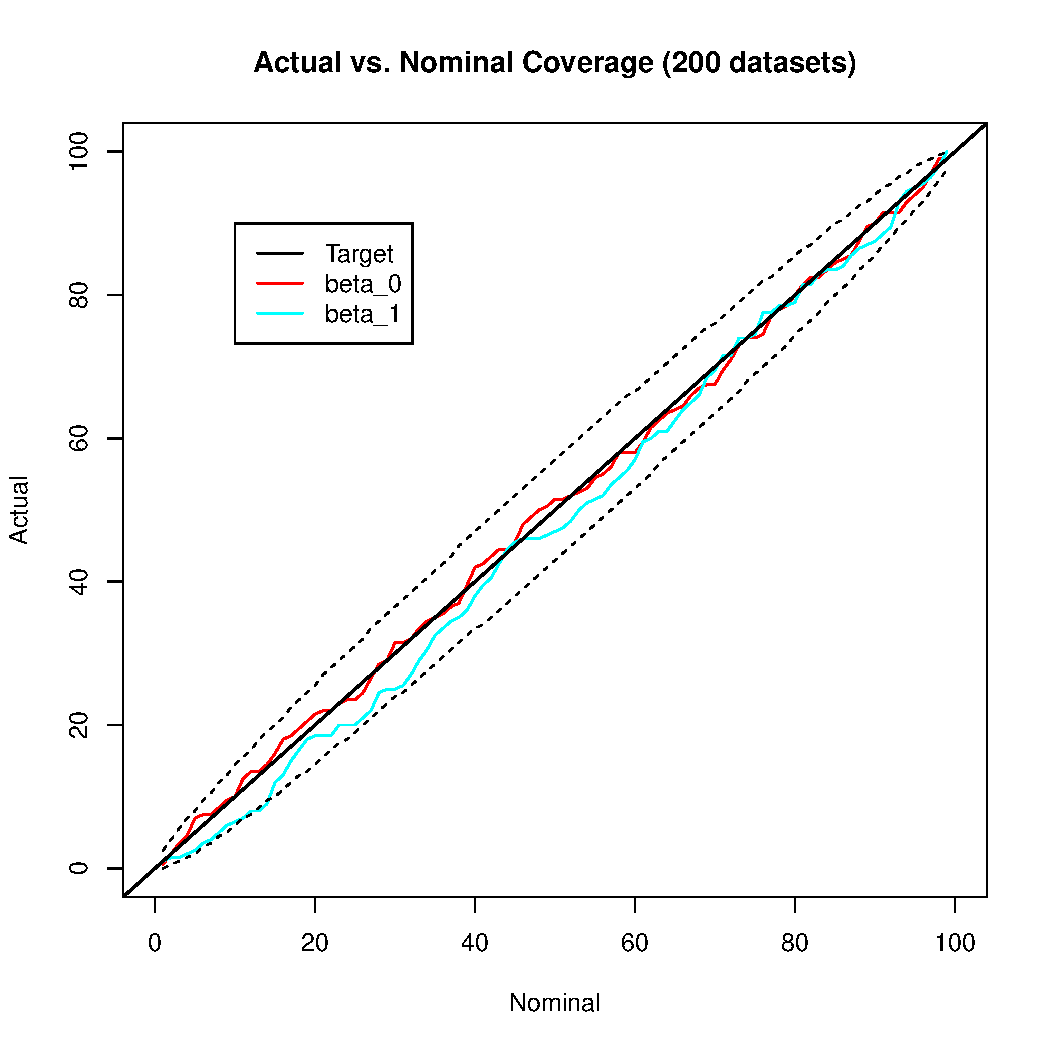
\includegraphics[width=4in]{BayesLogit/coverage_line_plot.pdf} 
   \caption{The actual coverage is very close to the nominal coverage for both target parameters. This guarantees that the Metropolis within Gibbs Sampler has been implemented correctly and that the Markov Chain has converged to its stationary distribution. }
   \label{fig:coverage-q2}
\end{figure}

\section*{Question 3: The breast cancer data set}
\subsection*{Fitting the Bayes logistic regression model}
The data was standardized to have zero mean and equal scale to aid in convergence of the chains because the scale between some covariates was very dramatic. The same MWG algorithm was applied to the breast cancer data, only here the dimension was eleven instead of two. Here we detail the only the specifications on the real data set that differ:
 
\begin{tabular}{ll}
\hline
Component & Description \\
\hline
Post Burn-in Chain Length & 80,000 \\
Burnin Length & 20,000 \\
\end{tabular}

All but two coefficients of $\beta \in \mathbb{R}^11 $ demonstrated some degree of convergence. The trace plots and posterior densities are shown  below.

 \begin{figure}[htbp] %  figure placement: here, top, bottom, or page
   \centering
   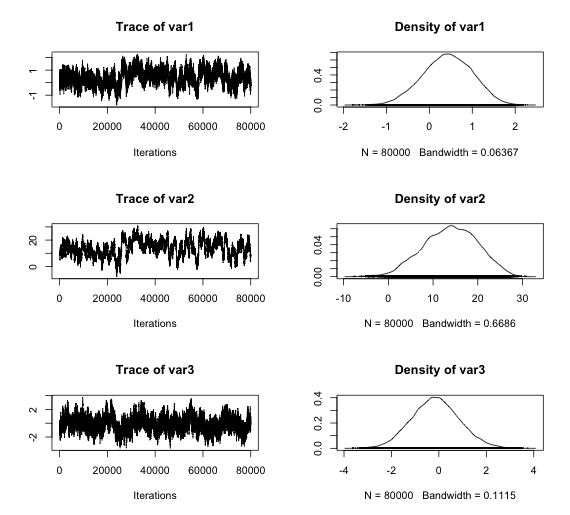
\includegraphics[width=2in]{BayesLogit/real_trace_1_3.png} 
   \caption{Trace and posterior densities of $\beta_1, \beta_2, \beta_3$}
\end{figure}

 \begin{figure}[htbp] %  figure placement: here, top, bottom, or page
   \centering
   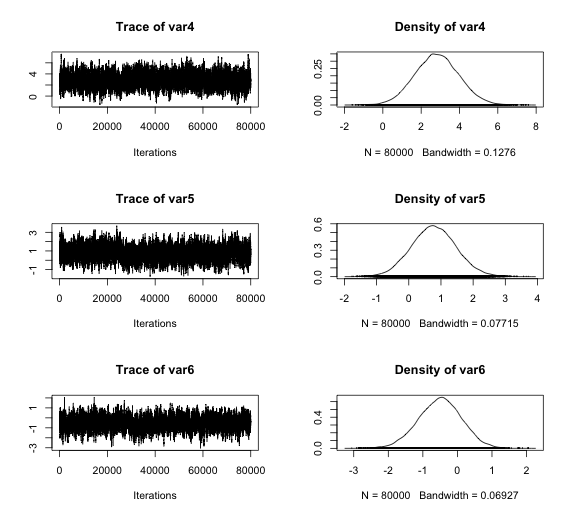
\includegraphics[width=2in]{BayesLogit/real_trace_4_6.png} 
   \caption{Trace and posterior densities of $\beta_4, \beta_5, \beta_6$}
\end{figure}


 \begin{figure}[htbp] %  figure placement: here, top, bottom, or page
   \centering
   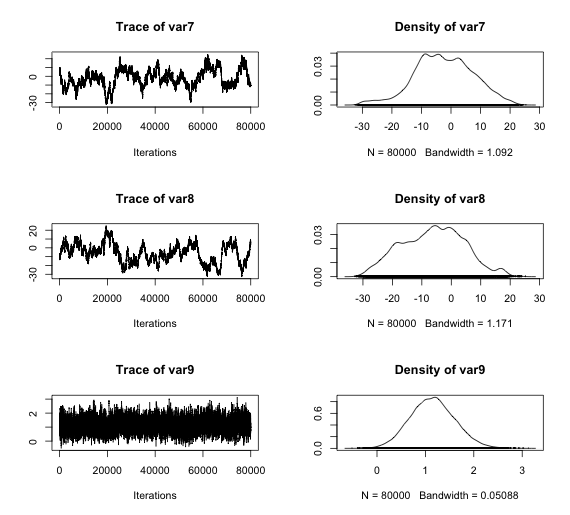
\includegraphics[width=2in]{BayesLogit/real_trace_7_9.png} 
   \caption{Trace and posterior densities of $\beta_7, \beta_8, \beta_9$}
\end{figure}

 \begin{figure}[htbp] %  figure placement: here, top, bottom, or page
   \centering
   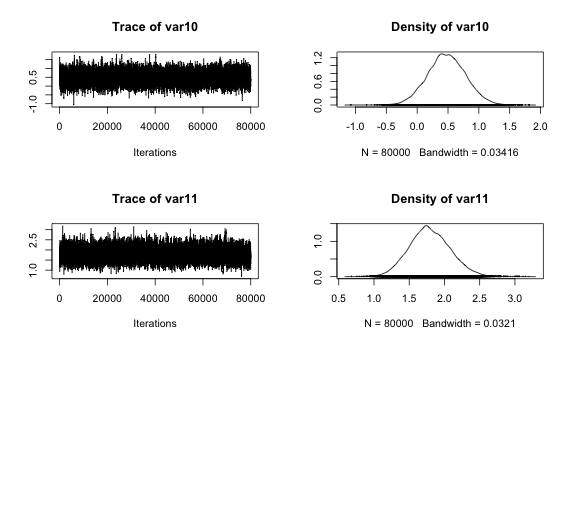
\includegraphics[width=2in]{BayesLogit/real_trace_10_11.png} 
   \caption{Trace and posterior densities of $\beta_{10}, \beta_{11}$}
\end{figure}

Interestingly, the glm standard error of the coefficients on area, perimeter, and radius, are much larger than the other coefficients (note that these are all measures on size). Correspondingly, the chains have difficulty converging on these parameters even when the proposal variance is increased by a factor of two upon initialization.  All other coefficients attain good convergence. The acceptance rates are all within a tolerable range. 

% latex table generated in R 3.0.0 by xtable 1.7-1 package
% Mon Oct 28 10:25:07 2013
\begin{table}[ht]
\centering
\caption{Percent Acceptance of the MCMC}
\begin{tabular}{rrrrrrrrrrrr}
  \hline
 & var1 & var2 & var3 & var4 & var5 & var6 & var7 & var8 & var9 & var10 & var11 \\ 
  \hline
1 & 42.77 & 38.16 & 51.67 & 45.04 & 48.03 & 37.98 & 56.76 & 31.97 & 49.99 & 41.44 & 40.90 \\ 
   \hline
\end{tabular}
\end{table}

\subsection*{lag-1 Autocorrelation}
Mixing is a way of saying how well the chain explored the parameter space. The autocorrelation is an indication of how good the Markov Chain was mixed; high autocorrelations suggests poor mixing (\url{http://stat.duke.edu/courses/Fall10/sta290/Lectures/Diagnostics/param-diag.pdf})

 \begin{figure}[htbp] %  figure placement: here, top, bottom, or page
   \centering
   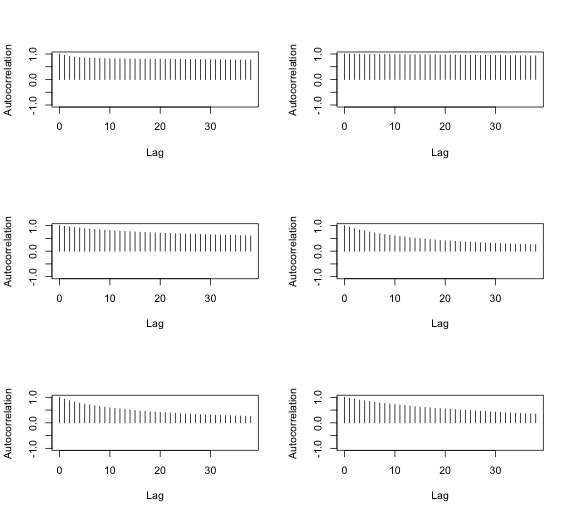
\includegraphics[width=2in]{BayesLogit/real_auto_cor_1_6.png} 
   \caption{Auto-correlation variables 1-6}
\end{figure}


 \begin{figure}[htbp] %  figure placement: here, top, bottom, or page
   \centering
   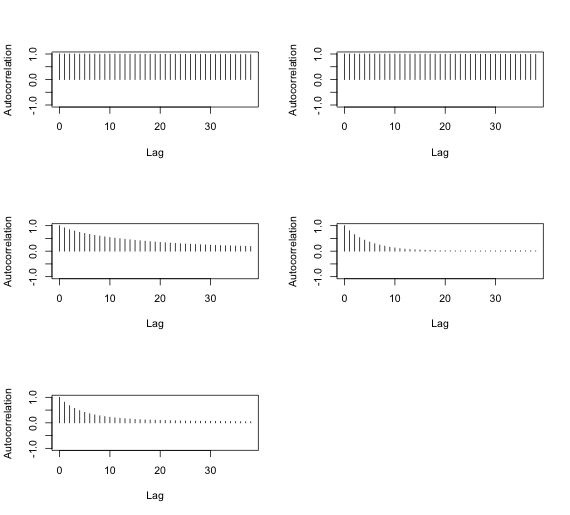
\includegraphics[width=2in]{BayesLogit/real_auto_cor_7_11.png} 
   \caption{Auto-correlation variables 7-11}
\end{figure}


The autocorrelation plots shows that $\beta_1,\beta_2,  \beta_7, \beta_8$ do not mix as well as we would like.  Thinning may reduce autocorrelation at the cost of posterior sample size and is only an option when the MC converges. Since good  mixing was not attained for all target parameters, we did not thin the posterior sample (\url{http://support.sas.com/documentation/cdl/en/statug/63033/HTML/default/viewer.htm#statug_introbayes_sect007.htm}). 

% latex table generated in R 3.0.0 by xtable 1.7-1 package
% Mon Oct 28 09:55:03 2013
\begin{table}[ht]
\centering
\caption{The lag-1 autocorrelation for each $\beta$}
\begin{tabular}{rrrrrrrrrrrr}
  \hline
 & beta1 & beta2 & beta3 & beta4 & beta5 & beta6 & beta7 & beta8 & beta9 & beta10 & beta11 \\ 
  \hline
1 & 0.94 & 0.89 & 0.09 & 0.21 & -0.28 & -0.09 & 0.11 & -0.54 & -0.03 & -0.02 & 0.03 \\ 
  2 & 0.89 & 1.00 & 0.26 & 0.20 & -0.30 & -0.20 & -0.01 & -0.48 & 0.03 & -0.01 & 0.15 \\ 
  3 & 0.09 & 0.26 & 0.97 & -0.06 & -0.07 & -0.63 & -0.65 & 0.41 & -0.10 & -0.17 & -0.05 \\ 
  4 & 0.21 & 0.20 & -0.05 & 0.94 & -0.62 & 0.19 & -0.19 & 0.04 & -0.60 & 0.01 & 0.13 \\ 
  5 & -0.29 & -0.30 & -0.06 & -0.60 & 0.93 & -0.30 & -0.04 & 0.20 & 0.54 & -0.06 & 0.06 \\ 
  6 & -0.09 & -0.21 & -0.63 & 0.19 & -0.29 & 0.96 & 0.15 & 0.01 & -0.25 & 0.04 & 0.04 \\ 
  7 & 0.11 & -0.01 & -0.65 & -0.19 & -0.04 & 0.15 & 1.00 & -0.87 & 0.21 & 0.07 & -0.06 \\ 
  8 & -0.54 & -0.48 & 0.41 & 0.04 & 0.20 & 0.00 & -0.87 & 1.00 & -0.16 & -0.04 & 0.00 \\ 
  9 & -0.03 & 0.03 & -0.10 & -0.58 & 0.54 & -0.24 & 0.20 & -0.16 & 0.91 & -0.13 & 0.29 \\ 
  10 & -0.02 & -0.01 & -0.16 & 0.02 & -0.05 & 0.06 & 0.07 & -0.04 & -0.10 & 0.80 & 0.19 \\ 
  11 & 0.04 & 0.15 & -0.05 & 0.12 & 0.05 & 0.04 & -0.06 & 0.00 & 0.28 & 0.17 & 0.81 \\ 
   \hline
\end{tabular}
\end{table}

\subsection*{Covariates related to cancer diagnosis}
An informal way of determining association of traits with cancer diagnosis is checking to see if 0 is contained in the 95\% posterior credible intervals. Intervals not containing zero are informally said to be related to cancer diagnosis. In particular, the cytology covariates related to cancer diagnosis are area, concavepts, smoothness, \& texture. 

% latex table generated in R 3.0.0 by xtable 1.7-1 package
% Mon Oct 28 10:30:31 2013
\begin{table}[ht]
\centering
\caption{95\% Posterior Credible Intervals of the coefficients in the Bayes logistic regression.}
\begin{tabular}{rrrrrrrrrrrr}
  \hline
 & beta1 & beta2 & beta3 & beta4 & beta5 & beta6 & beta7 & beta8 & beta9 & beta10 & beta11 \\ 
  \hline
2.5\% & -0.71 & 2.02 & -2.08 & 0.60 & -0.56 & -1.75 & -23.40 & -26.06 & 0.27 & -0.12 & 1.25 \\ 
  97.5\% & 1.50 & 24.97 & 1.90 & 5.11 & 2.19 & 0.69 & 16.40 & 15.15 & 2.08 & 1.09 & 2.38 \\ 
Contains zero & yes & no & yes & no & yes & yes & yes & yes & no & yes & no \\
   \hline
\end{tabular}
\end{table}
\subsection*{Goodness of fit}

The posterior predictive checks on the sample mean and standard deviation have posterior predictive p-value very close to 1. That is to say, the Bayes logistic regression model fits the data very well. The posterior predictive method simulates data by sampling the posterior target parameters. We would expect a summary statistic on the real data to be in the same neighborhood of summary statistics of the simulated data if the posterior target parameters of the model are correctly representing the key information about the process generating the real data; hence a good model fit.
\begin{figure}[htbp] %  figure placement: here, top, bottom, or page
   \centering
   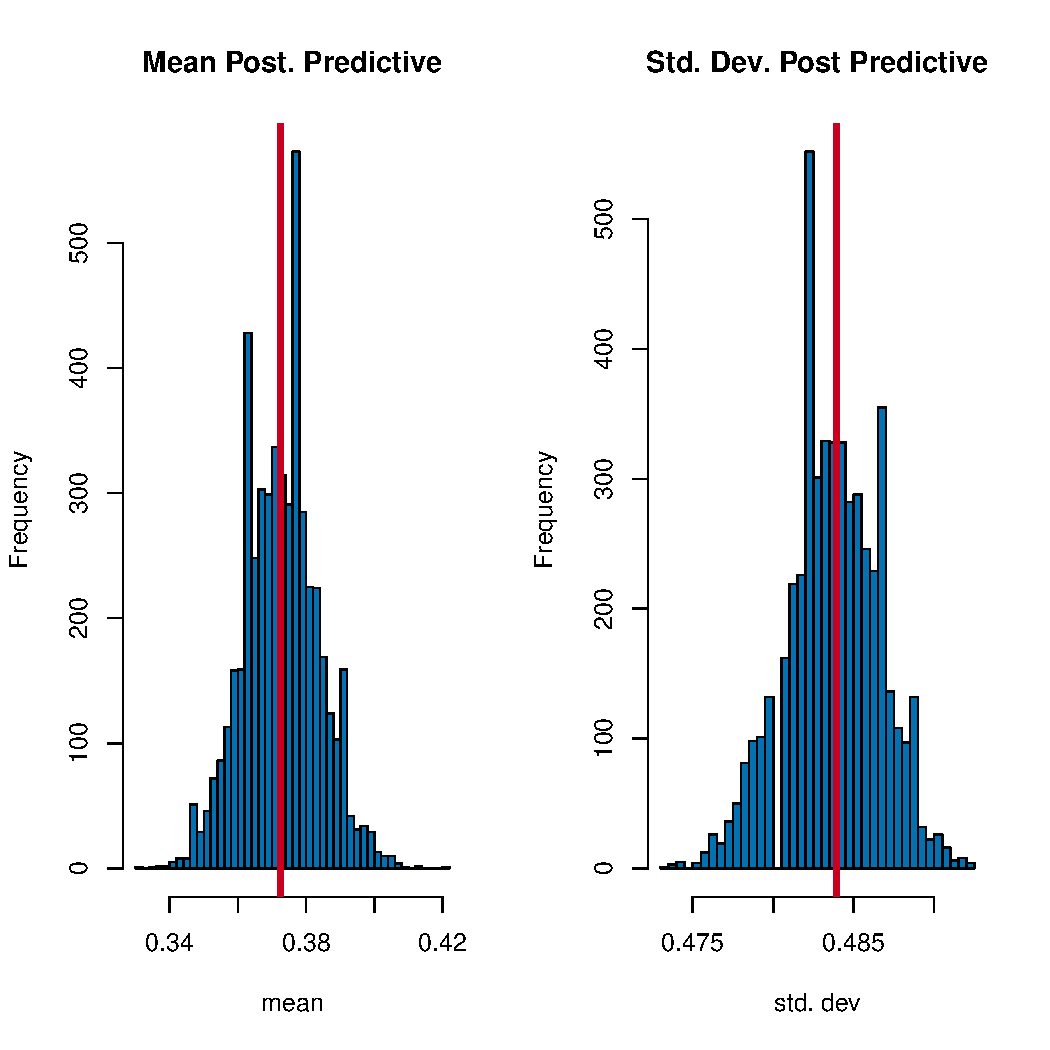
\includegraphics[width=4in]{BayesLogit/real_data_posterior_predictive.pdf} 
   \caption{The posterior predictive check on the mean and standard deviation, respectively for 5,000 simulated data sets. The red line indicates the real data sample mean and standard deviation location, which is compared to the  simulated data summary statistics in the blue histogram.}
   \label{fig:coverage-q2}
\end{figure}

\newpage
\section*{Appendix A: Metropolis within Gibbs Code}

\begin{verbatim}
library(mvtnorm)

log.posterior <- function(mu.0, Sigma.0.inv, beta, y, m, X) {  
  #key functions
  log.prior <- function(mu.0, Sigma.0.inv, beta) {
    log( dmvnorm(x = beta, mean = mu.0, sigma = Sigma.0.inv) )
  }
  
  log.lik <- function(beta, y, m, X) {
    expit <- function(x, beta) {
      eEta <- exp( x %*% beta) 
      eEta / (1 + eEta)
    }
    sum( log( dbinom(x = y, size = m, prob = expit(X,beta)) ) )
  }
  log.prior(mu.0, Sigma.0.inv, beta) + log.lik(beta, y, m, X)
}


proposal <- function(theta.t, sd.tune) {
  rnorm(n = 1, mean = theta.t, sd = sd.tune)
}


check.proposal.var <-function(n.accept, n.iter.block , psd, 
                              verbose) {
  stopifnot(length(psd) == length(n.accept))
  if (verbose) {
    print("------------Retuned Parameters------------")
    print("Original:")
    print(psd)  
  }
  
  for (k in seq_along(psd)) {
    arate <- n.accept[k]/n.iter.block
    if (verbose) {
      print("Current Acceptance Rate:")
      print(arate)  
    }
    
    if (arate < 0.1) {
      psd[k] <- psd[k]*0.25
    } else if (0.1 <= arate & arate < 0.3) {
      psd[k] <- psd[k]*0.5
    } else if (0.6 < arate & arate <= 0.9) {
      psd[k] <- psd[k]*2
    } else if (arate > 0.9) {
      psd[k] <- psd[k]*4
    } else{
      #no retuning necessary for kth proposal variance
    }
  }
  if (verbose){
    print("Retuned:")
    print(psd)  
  }
  return(psd)
}

"bayes.logreg" <- function(m,y,X,beta.0,Sigma.0.inv,
                           niter=10000,burnin=1000,
                           print.every=1000,retune=100,
                           verbose=TRUE){
  
  #GLM aids in selecting priors
  mod.glm <- glm( cbind(y, m -y) ~ . , data = as.data.frame(X[,-1]), family = binomial(link = "logit"))
  #prior mean on beta
  mu.0 <- summary(mod.glm)$coefficients[,1]
  #proposal standard deviation (tuning parameter)
  psd <- summary(mod.glm)$coefficients[,2]

  #naive priors
  #mu.0 <- rep(0, times = length(beta.0))
  #psd <- rep(0.5, times = length(beta.0))
  
  #acceptance rate
  accept.count <- rep(0, times = length(beta.0))
  burnin.count <- rep(0, times = length(beta.0))
  retune.check.index <- seq(from = retune, to = burnin, by = retune) 
  
  #print every
  progress.index <- seq(from = print.every, to = niter, by = print.every)
  #################################
  #metropolis hastings within gibbs
  #################################
  
  #container of markov chain for beta 
  beta.chain <- matrix(nrow = niter, ncol = length(beta.0))
  #initial state provided by user (should not matter what it is in the end)
  beta.current <- beta.0
  print("Percent completed:")
  for (t in seq_len(niter)) {
    
    if(any(progress.index == t)) {
      cat(paste(round(100*t/niter, 3), "\t")); flush.console();
    }
    
    #retune proposal variance checks (within burnin time)
    if (any(retune.check.index == t)) {
      psd <- check.proposal.var(n.accept = burnin.count, 
                                n.iter.block = retune , psd = psd,
                                verbose)
      #reset the count
      burnin.count <- rep(0, times = length(beta.0))
    }    
    
    for (j in seq_along(beta.current)) {
      
      #propose a new scalar candidate for beta.current[j]
      beta.prop <- proposal(theta.t = beta.current[j], sd.tune = psd[j])
      #only difference between candidate and current is the jth position
      beta.star <- beta.current
      beta.star[j] <- beta.prop 
      
      #decision to accept or reject
      log.alpha <- log.posterior(mu.0, Sigma.0.inv, beta.star, y, m, X) -
        log.posterior(mu.0, Sigma.0.inv, beta.current, y, m, X)
      log.u <- log(runif(n = 1))
      acceptance <- log.u < log.alpha
      
      #if(is.na(acceptance)) {
        
        #cat("Missing Value for acceptance at iteration:\t", t, "\n")
        #cat("Proposal:\t", beta.prop, "\n")
        #cat("log.alpha:\t", log.alpha, "\n")
      #}
      
      if (!is.na(acceptance) & acceptance) {
        #update the current beta for all subsequent dimensions of beta
        beta.current[j] <- beta.prop
        #keep separate accceptance rates
        if (burnin < t) {
          accept.count[j] <- accept.count[j] + 1
        } else {
          burnin.count[j] <- burnin.count[j] + 1 
        }
      } else {
        #reject proposal and keep current beta as is.
      }
    }
    #store the results of the metropois hastings within Gibbs for time point t
    beta.chain[t,] <- beta.current
  }
  cat("\n------------------------------\n"); flush.console();
  post.burnin.index <- (burnin + 1):niter
  
  print("Percent acceptance for each parameter:")
  print(round(100*accept.count/length(post.burnin.index), 3))  
  print("Tuned Proposal Variance Values")
  print(psd)
  return(beta.chain[post.burnin.index,])
}

post.predictive <- function(n.pred = 100, posterior, y, X, stat = mean) {
  
  n.post <- dim(posterior)[1]
  
  if(n.pred > n.post) {
    stop("Predictive data sets must be less than posterior samples")
  }
  
  pred.index <- sample(x = seq_len(n.post), size = n.pred)
  beta.post <- posterior[pred.index,]
  
  n.y <- length(y)
  sum.stats <- vector(mode  = "numeric", length = n.pred)
  
  expit <- function(x, beta) {
    eEta <- exp( x %*% beta) 
    eEta / (1 + eEta)
  }
  
  for (j in seq_len(n.pred)) {
    pred.data <- rbinom(n = n.y, size = 1, prob = expit(X,beta.post[j,]))
    sum.stats[j] <- stat(pred.data)
  } 
  sum.stats
}

\end{verbatim}


\newpage
\section*{Appendix B: Question 2 Script}
\begin{verbatim}

##
#
# Logistic regression
# 
# Y_{i} | \beta \sim \textrm{Bin}\left(n_{i},e^{x_{i}^{T}\beta}/(1+e^{x_{i}^{T}\beta})\right)
# \beta \sim N\left(\beta_{0},\Sigma_{0}\right)
#
##

library(mvtnorm)
library(coda)

########################################################################################
########################################################################################
## Handle batch job arguments:

# 1-indexed version is used now.
args <- commandArgs(TRUE)

cat(paste0("Command-line arguments:\n"))
print(args)

####
# sim_start ==> Lowest simulation number to be analyzed by this particular batch job
###

#######################
sim_start <- 1000
length.datasets <- 200
#######################

if (length(args)==0){
  sinkit <- FALSE
  sim_num <- sim_start + 46
  set.seed(1330931)
} else {
  # Sink output to file?
  sinkit <- TRUE
  # Decide on the job number, usually start at 1000:
  sim_num <- sim_start + as.numeric(args[1])
  # Set a different random seed for every job number!!!
  set.seed(762*sim_num + 1330931)
}

# Simulation datasets numbered 1001-1200

########################################################################################
########################################################################################

#The core Metropolis within Gibbs algorithm is written in this file
source("BLR_metropolis_within_gibbs.R")
#################################################
# Set up the specifications:
beta.0 <- c(0,0)
p <- 2
Sigma.0.inv <- diag(rep(1.0,p))
# etc... (more needed here)
#################################################

# Read data corresponding to appropriate sim_num:
sim_data_file <- paste("data/blr_data_", sim_num, ".csv", sep = "")
data <- read.csv(file = sim_data_file)

# Extract X and y:
m <- data$n
y <- data$y
X <- as.matrix(data[,3:4])

# Fit the Bayesian model:
beta.chain <- bayes.logreg(m = m,y = y,X  = X,
                           beta.0 = beta.0, Sigma.0.inv = Sigma.0.inv,
                           niter=20000, burnin=5000,
                           print.every=1000, retune=100, verbose=FALSE)

# Extract posterior quantiles...
posterior.quantiles <- apply(beta.chain , MARGIN = 2, FUN = quantile, 
                             probs = seq(from = 0.01, to = 0.99, by = 0.01))
posterior.quantiles
# Write results to a (99 x p) csv file...
result_data_file <- paste("results/blr_res_", sim_num, ".csv", sep = "")
write.table(x = as.data.frame(posterior.quantiles), file = result_data_file, 
            row.names=FALSE, col.names=FALSE, sep=",")
# Go celebrate.

cat("done. :)\n")
#

#diagnostics
#library(MCMCpack)
#mcmc.beta.chain <- mcmc(beta.chain)
#plot(mcmc.beta.chain)
#
autocorr.plot(mcmc.beta.chain)

acf(mcmc.beta.chain)

\end{verbatim}

\newpage
\section*{Appendix C: Question 3 Script}

\begin{verbatim}

########################
#working directory & start clean
rm(list = ls())
setwd("~/myrepos//sta250/Stuff/HW1/BayesLogit/")
########################

#####################################
#read in #cancer data set
#parse it to meaningful
#objects in terms of {m, y, X}

data <- read.table("breast_cancer.txt", header = TRUE)#, na.strings = "?")

#check that there are no missing values, otherwise send error message
check.missing <- na.fail(data)
#this data is not in grouped format as the previous simulation
m  <- rep(1, times = dim(data)[1])
#Call malignant cases as "success" and redefine response in terms of {1,0}
y <- ifelse(data$diagnosis == "M", 1, 0)
covariate.index <- 1:10
X <- cbind(rep(1, times = dim(data)[1]), scale(as.matrix(data[,covariate.index])))
colnames(X) <- c("intercept", names(data)[covariate.index])
####################################

#################################################
# Set up the model specifications:
p <- dim(X)[2]
beta.0 <- rep(0, times = p)
Sigma.0.inv <- diag(rep(1000,p))
#################################################

##################################################
#Load the key algorithmic functions
source("BLR_metropolis_within_gibbs.R")
##################################################


######################################################################
# Fit the Bayesian model:
beta.chain <- bayes.logreg(m = m,y = y,X  = X,
                           beta.0 = beta.0, Sigma.0.inv = Sigma.0.inv,
                           niter=5e4, burnin=2e4,
                           print.every=1000, retune=500, verbose=FALSE)
#####################################################################

#save the results
#save(list = ls(), file = "real_data_output_long.rda")


#########################################################################
#diagnostics
load("real_data_output_long.rda")

######################################################################
#trace plot diagnostics

library(MCMCpack)
library(coda)
mcmc.beta.chain <- mcmc(beta.chain)
plot(mcmc.beta.chain)
effectiveSize(mcmc.beta.chain)
#acceptance rates
acc.rate <- 100*(1 - rejectionRate(mcmc.beta.chain))
acc.rate.mat <- matrix(acc.rate, nrow = 1, ncol = 11)
colnames(acc.rate.mat) <- names(acc.rate)
library(xtable)
xtable(acc.rate.mat)

#autocorrelation
autocorr.plot(mcmc.beta.chain)
#lag 1
beta.ac1 <- sapply(1:p, function(i) autocorr(mcmc.beta.chain, lags = 1)[,,i])

beta.ac1 <- as.data.frame(beta.ac)
names(beta.ac1) <- paste("beta", 1:11, sep = "")
xtable(beta.ac1)

######################################################################
#experimental: thinning the mcmc chain
thin.index <- seq(from = 1, to = 8e4, by = 5)

thin.beta.chain <- beta.chain[thin.index,]
mcmc.thin.beta.chain <- mcmc(thin.beta.chain)
autocorr.plot(mcmc.beta.chain)


######################################################################
# Extract posterior quantiles...
posterior.quantiles <- apply(beta.chain , MARGIN = 2, FUN = quantile, 
                             probs = c(0.025, 0.975))
colnames(posterior.quantiles) <- paste("beta", 1:11, sep = "")
xtable(posterior.quantiles)
######################################################################

######################################################################
#posterior predictive analysis
pdf("real_data_posterior_predictive.pdf")
beta.post.pred.mean <- post.predictive(n.pred = 5000, posterior = beta.chain, y = y, X = X, 
stat = mean)
beta.post.pred.sd <- post.predictive(n.pred = 5000, posterior = beta.chain, y = y, X = X, 
stat = sd)
par(mfrow = c(1,2))
library(RColorBrewer)
brew.col <- brewer.pal(n = 4, "RdBu")
hist(beta.post.pred.mean, 40, col = brew.col[4], 
       main = "Mean Post. Predictive", xlab = "mean")
abline(v = mean(y), col  = brew.col[1], lwd = 4)
hist(beta.post.pred.sd, 40, col = brew.col[4], 
        main = "Std. Dev. Post Predictive", xlab = "std. dev")
abline(v = sd(y), col  = brew.col[1], lwd = 4)
dev.off()
######################################################################


\end{verbatim}

\end{document}  
